\chapter{Thiết kế hệ thống}

\section{Tổng quan kiến trúc hệ thống}

Hệ thống được thiết kế theo hướng tách biệt rõ giữa giao diện người dùng,
logic nghiệp vụ, pipeline AI và hạ tầng lưu trữ. Mục tiêu của kiến trúc là
cho phép thay đổi LLM provider, vector database, graph database hoặc LMS mà
không phải viết lại use case cốt lõi.

\begin{figure}[H]
    \centering
    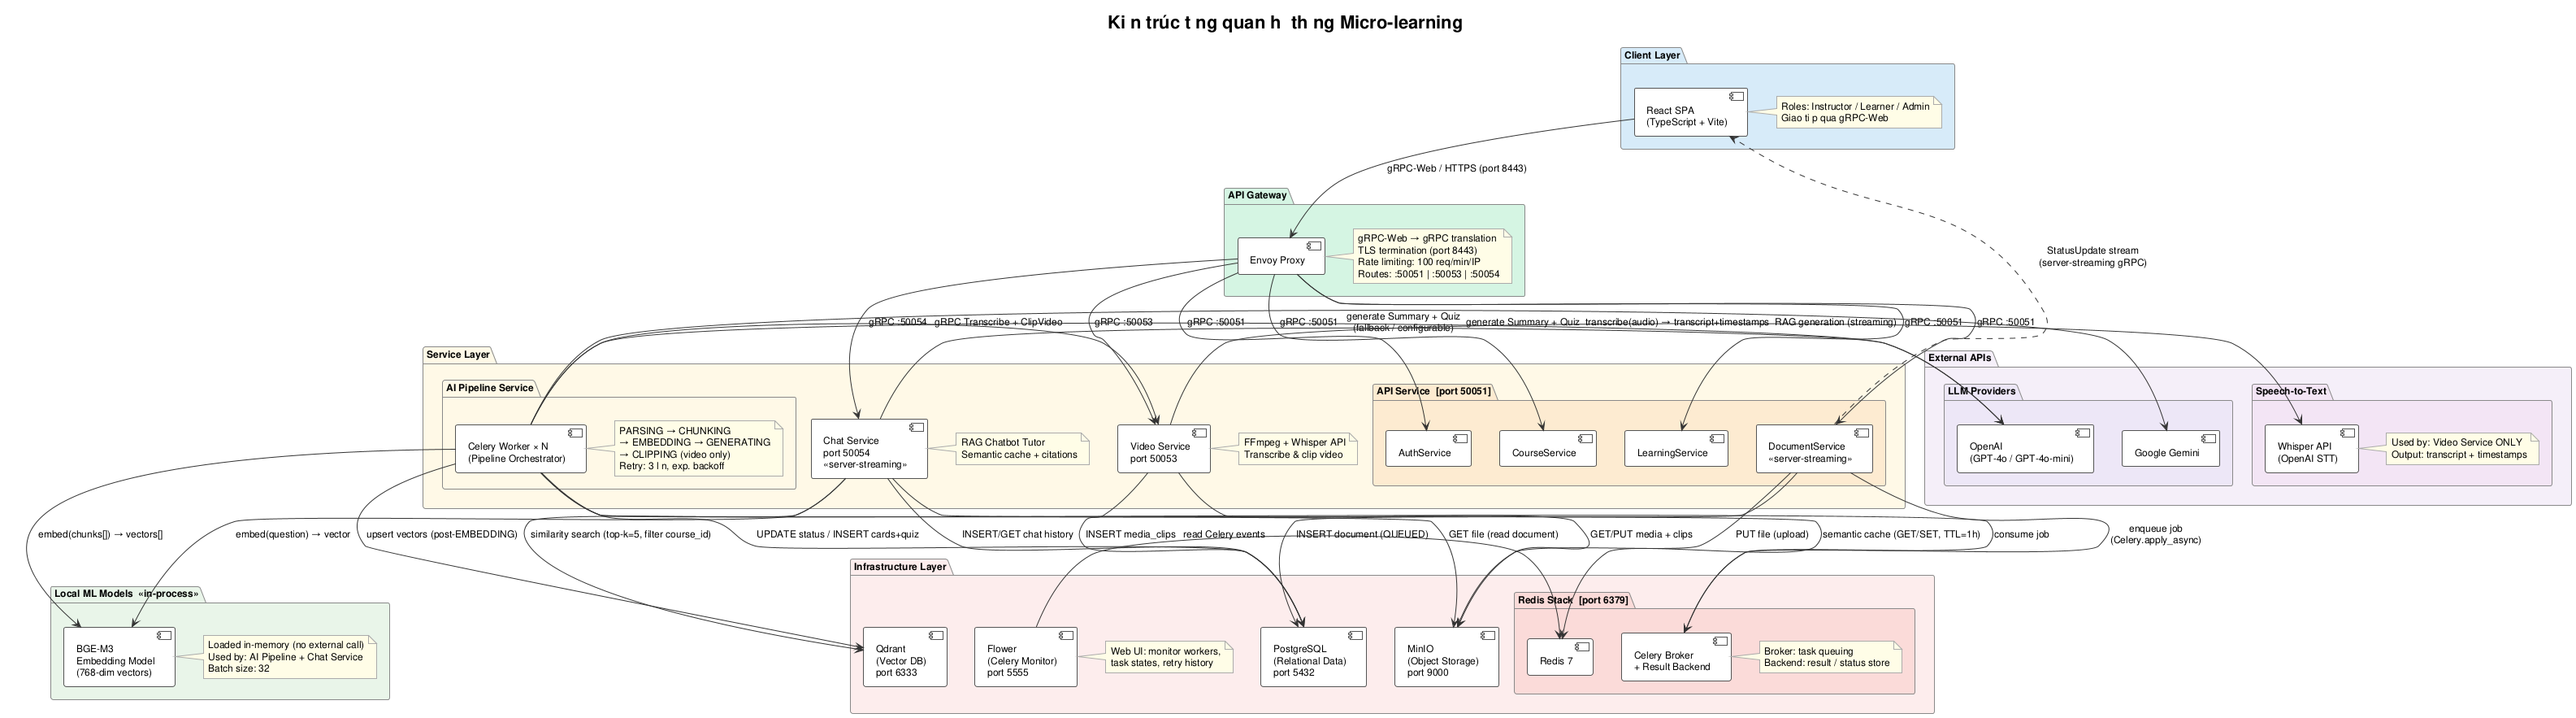
\includegraphics[width=0.95\textwidth]{diagrams/arch_overview.png}
    \caption{Tổng quan kiến trúc hệ thống.}
    \label{fig:arch-overview-lvtn}
\end{figure}

Các lớp chính trong hệ thống gồm:
\begin{itemize}
    \item \textbf{LMS layer:} Open edX hoặc Moodle đóng vai trò nền tảng học
          tập chính, gọi hệ thống qua LTI 1.3.
    \item \textbf{Frontend layer:} Next.js cung cấp màn hình review cho giảng
          viên, màn hình học cho học viên và route xử lý LTI.
    \item \textbf{Application/API layer:} Python gRPC service expose các use
          case như upload/process/search/get quiz/ingest curriculum.
    \item \textbf{Worker layer:} document worker, enrichment worker và outbox
          worker xử lý bất đồng bộ.
    \item \textbf{Storage layer:} PostgreSQL lưu metadata, MinIO lưu file,
          Qdrant lưu vector, Neo4j lưu Knowledge Graph.
    \item \textbf{AI provider layer:} LLM và embedding model được gọi qua
          adapter để giảm phụ thuộc vào provider cụ thể.
\end{itemize}

Backend AI áp dụng Hexagonal Architecture. Domain/application layer chứa các
entity và use case cốt lõi; ports định nghĩa interface cho parser, chunker,
embedder, vector store, graph store, metadata store và LLM client; adapters
hiện thực giao tiếp với PostgreSQL, Qdrant, Neo4j, MinIO, Redis và provider
AI.

\begin{figure}[H]
    \centering
    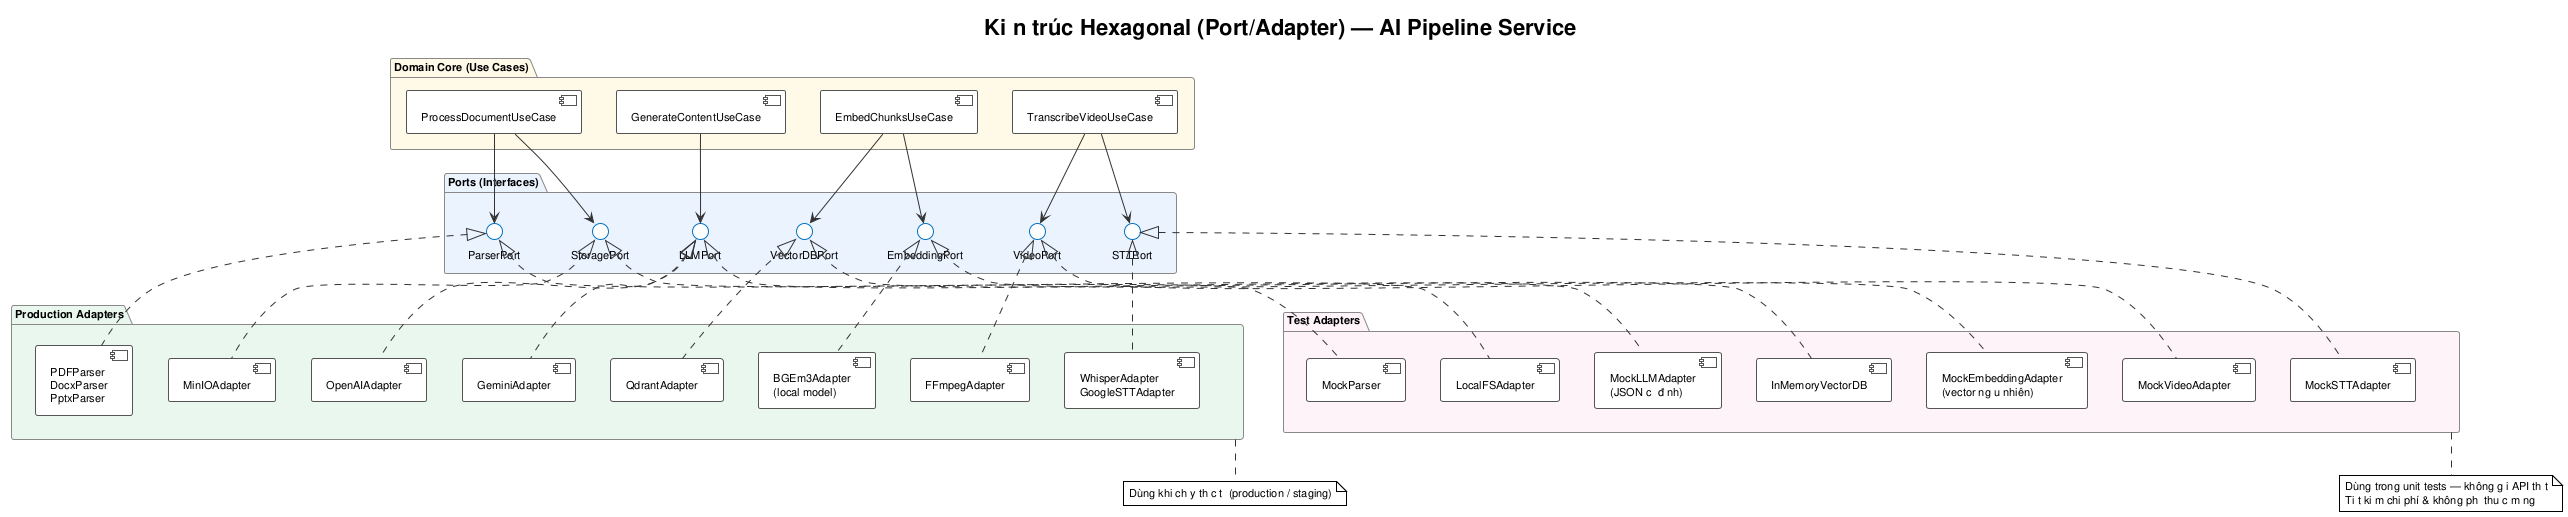
\includegraphics[width=0.95\textwidth]{diagrams/arch_hexagonal.png}
    \caption{Kiến trúc Hexagonal trong backend AI.}
    \label{fig:hexagonal-lvtn}
\end{figure}

\section{Kiến trúc tích hợp LMS}

\subsection{Open edX / Moodle}

Open edX là nền tảng tích hợp chính trong phạm vi hiện tại. Hệ thống được
nhúng vào khóa học thông qua LTI 1.3. Khi học viên hoặc giảng viên mở activity
từ Open edX, LMS gửi LTI launch request đến frontend. Frontend xác thực
request, tạo session và điều hướng đến màn hình phù hợp với vai trò người
dùng.

Moodle được phân tích như hướng triển khai tương thích. Vì hệ thống đóng vai
trò LTI Tool Provider, về nguyên tắc có thể đăng ký như external tool trong
Moodle mà không cần thay đổi lõi backend. Sự khác biệt chủ yếu nằm ở cấu hình
platform, deployment ID, client ID, keyset URL và mapping role/context.

\subsection{LTI 1.3 Flow}

\begin{figure}[H]
    \centering
    
\includegraphics[width=0.95\textwidth]{figures/lti_auth_flow.png}
    \caption{Luồng xác thực LTI 1.3/OIDC.}
    \label{fig:lti-flow-lvtn}
\end{figure}

Hệ thống hoạt động như LTI Tool. Khi người dùng click từ LMS, LMS khởi tạo
OIDC login, sau đó gửi LTI launch request chứa JWT đã ký. Frontend/route LTI
kiểm tra issuer, client ID, deployment ID, nonce, signature và claim người
dùng. Sau khi xác thực, hệ thống tạo session nội bộ và điều hướng người dùng
đến màn hình tương ứng.

\subsection{Vai trò LMS trong hệ thống}

LMS giữ vai trò quản lý khóa học, danh sách người dùng, phân quyền ban đầu và
điểm truy cập học tập. Hệ thống AI không thay thế LMS mà bổ sung một tool bên
ngoài để tạo và phân phối Micro-Content/Quiz. Thiết kế này giúp giảm rủi ro
triển khai vì cơ sở đào tạo vẫn có thể giữ quy trình LMS hiện hữu.

\section{Thiết kế AI Pipeline}

\subsection{Trích xuất tài liệu}

Sau khi giảng viên upload file, backend lưu file gốc vào MinIO và tạo metadata
document trong PostgreSQL. Worker nhận job từ queue, tải file và chọn parser
theo định dạng. Parser trích xuất text, heading, page range và metadata cần
thiết để phục vụ chunking và truy xuất nguồn về sau.

\subsection{OCR}

OCR được đặt sau bước phát hiện text layer. Nếu PDF có text layer đủ chất
lượng, hệ thống đọc trực tiếp văn bản. Nếu PDF là ảnh hoặc lượng text trích
xuất quá ít, pipeline chuyển sang OCR. Kết quả OCR cần lưu confidence để
giảng viên biết phần nào có nguy cơ sai khi review.

Trong phạm vi hiện tại, OCR production cho tài liệu scan chất lượng thấp được
xem là thiết kế mở rộng. Pipeline vẫn chừa adapter OCR để có thể bổ sung
Tesseract hoặc dịch vụ OCR chuyên biệt khi cần.

\subsection{Chunking}

Chunking chia tài liệu dài thành các đơn vị đủ nhỏ để embedding và đưa vào
prompt, nhưng vẫn đủ ngữ cảnh để giữ ý nghĩa học thuật. Hệ thống ưu tiên
heading-based chunking cho tài liệu có cấu trúc rõ. Mỗi chunk giữ heading path
như ``Chương 2 > 2.1 Khái niệm'', page range và document ID.

Với tài liệu thiếu heading, hệ thống dùng fallback chunking theo kích thước
token/ký tự và overlap. Overlap giúp giảm rủi ro cắt mất thông tin giữa hai
chunk liên tiếp nhưng cần được cấu hình hợp lý để tránh tăng chi phí embedding
và LLM.

\subsection{Embedding}

Mỗi chunk sau khi tạo được chuyển thành embedding bằng mô hình đa ngôn ngữ.
Vector được lưu vào Qdrant cùng payload metadata như course ID, document ID,
chunk ID, heading path, language và page range. Metadata này cho phép hệ thống
lọc retrieval theo khóa học, tài liệu hoặc chương.

\subsection{Retrieval}

Retrieval được dùng cho semantic search, RAG chatbot và sinh quiz theo LO.
Luồng truy xuất gồm embed query, tìm top-K chunk trong Qdrant, lọc theo
metadata và tăng ưu tiên bằng quan hệ Knowledge Graph nếu có. Với LMS, bước
lọc theo course/context là bắt buộc để tránh truy xuất nhầm nội dung ngoài
quyền truy cập của người học.

\subsection{Generation}

LLM generation nhận prompt gồm instruction, context chunk, Learning Outcome,
Bloom level, số lượng câu hỏi và schema đầu ra. Nội dung sinh ra được validate
theo JSON schema, rule nghiệp vụ và liên kết nguồn. Kết quả hợp lệ được lưu
như bản nháp để giảng viên review; hệ thống không publish tự động nội dung do
AI sinh ra.

\section{Thiết kế lưu trữ và dữ liệu}

\subsection{PostgreSQL}

PostgreSQL là source of truth cho dữ liệu nghiệp vụ. Các nhóm bảng chính gồm:
\begin{itemize}
    \item \textbf{Document:} document, file metadata, trạng thái pipeline.
    \item \textbf{Chunking:} chunk content, heading path, vị trí trong tài
          liệu, metadata ngôn ngữ.
    \item \textbf{Generated content:} lesson card, quiz item, đáp án, giải
          thích, trạng thái review.
    \item \textbf{Curriculum:} course, chapter, learning outcome, assessment,
          mapping LO-assessment và chunk-LO.
    \item \textbf{Learning data:} progress, quiz submission, score và event
          học tập.
\end{itemize}

\begin{figure}[H]
    \centering
    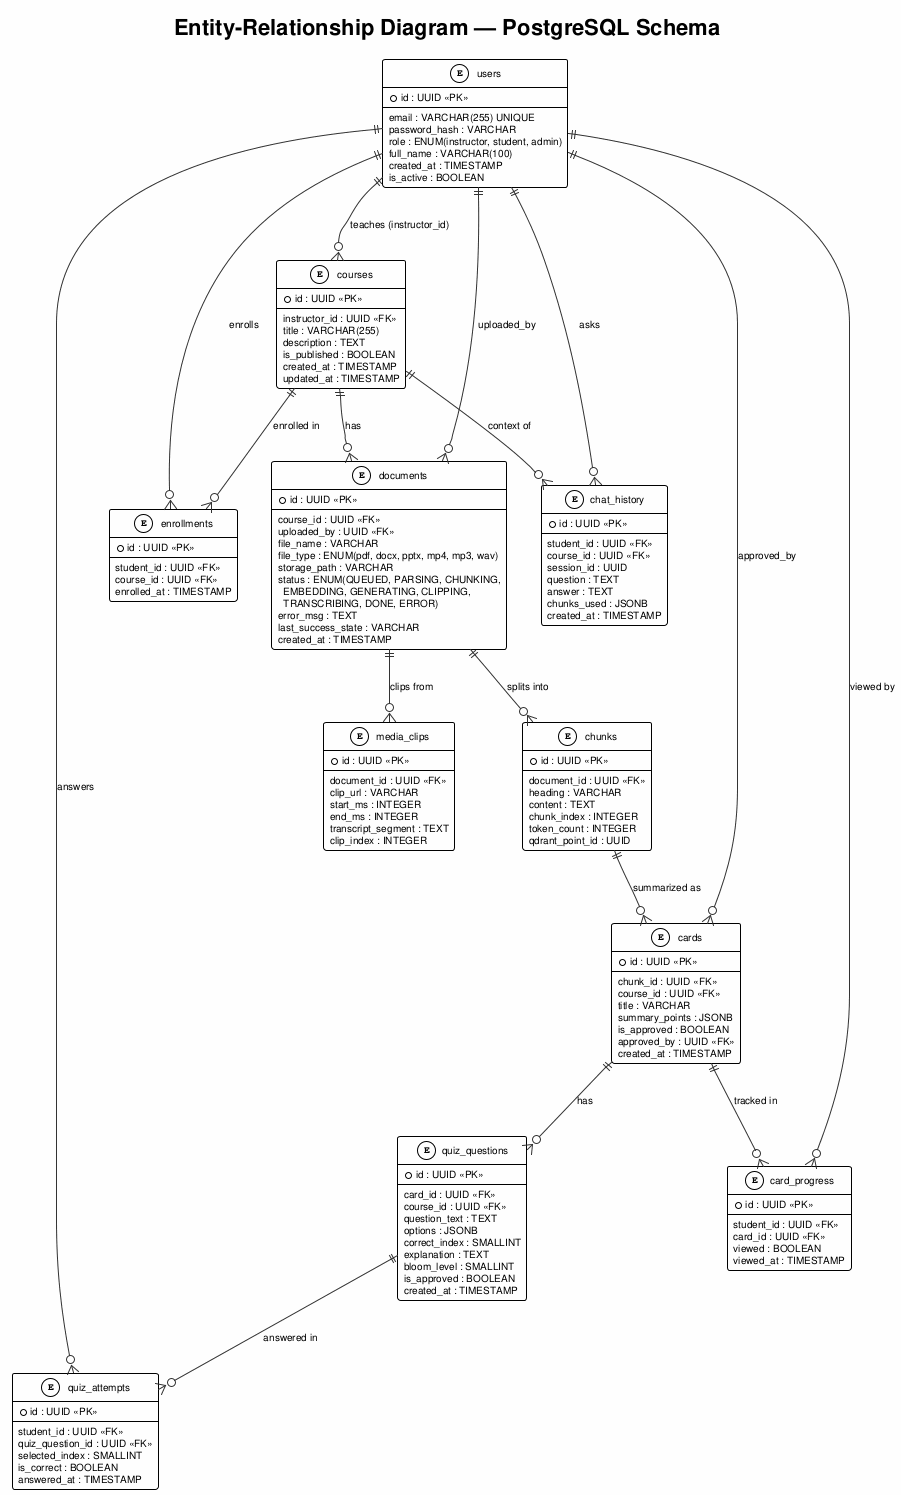
\includegraphics[width=0.95\textwidth,height=0.78\textheight,keepaspectratio]{diagrams/er_diagram.png}
    \caption{ER diagram của hệ thống.}
    \label{fig:er-lvtn}
\end{figure}

\subsection{Qdrant Vector DB}

Qdrant lưu vector embedding của chunk và payload metadata. Mỗi vector point
đại diện cho một chunk. Các thao tác chính gồm tạo collection theo kích thước
embedding, upsert vector sau khi chunking, search top-K theo query vector và
filter theo course, document hoặc language.

\subsection{Neo4j Graph DB}

Neo4j lưu projection Knowledge Graph cho curriculum. PostgreSQL vẫn giữ dữ
liệu gốc, còn Neo4j tối ưu cho truy vấn quan hệ tri thức như chunk nào hỗ trợ
LO nào, assessment nào đo LO nào hoặc chapter nào liên quan đến một nhóm
chuẩn đầu ra.

\subsection{MinIO / Object Storage}

MinIO lưu file gốc được upload bởi giảng viên. Metadata trong PostgreSQL chỉ
lưu đường dẫn object, checksum, MIME type, kích thước và trạng thái xử lý. Cách
tách này giúp database không phải lưu binary lớn và cho phép worker tải file
theo nhu cầu.

\subsection{Redis / Queue}

Redis và queue được dùng cho các job bất đồng bộ như parse document, sinh
embedding, gọi LLM và đồng bộ graph. Mỗi job cần lưu trạng thái, số lần retry,
thời điểm bắt đầu/kết thúc và lỗi cuối cùng để frontend có thể hiển thị tiến
trình cho giảng viên.

\section{Thiết kế mô hình tri thức và chiến lược truy xuất}

\subsection{Curriculum-aware Retrieval}

Curriculum-aware retrieval đưa thông tin chương trình học vào quá trình chọn
context. Khi giảng viên chọn một Learning Outcome hoặc chapter, hệ thống ưu
tiên chunk có quan hệ trực tiếp với LO/chapter đó trước khi đưa vào prompt.
Cách làm này giúp quiz bám mục tiêu học tập hơn so với chỉ dựa trên vector
similarity.

\subsection{GraphRAG Strategies}

GraphRAG trong luận văn được thiết kế theo ba mức:
\begin{enumerate}
    \item \textbf{Graph filtering:} chỉ lấy chunk có quan hệ với LO/chapter
          mục tiêu.
    \item \textbf{Graph-aware reranking:} kết hợp điểm vector similarity với
          điểm quan hệ trong graph.
    \item \textbf{Graph explanation:} lưu rationale để giải thích vì sao một
          chunk hoặc quiz liên quan đến LO.
\end{enumerate}

Reasoning đa bước trên graph được xem là hướng mở rộng, không trình bày như
kết quả hoàn thiện trong giai đoạn hiện tại.

\subsection{Metadata Strategy}

Metadata được lưu nhất quán giữa PostgreSQL, Qdrant và Neo4j. Các khóa quan
trọng gồm \texttt{course\_id}, \texttt{document\_id}, \texttt{chunk\_id},
\texttt{chapter\_id}, \texttt{lo\_id}, heading path, page range, language và
source version. Metadata giúp truy xuất có thể lọc theo phạm vi khóa học,
truy ngược nguồn và đánh giá chất lượng retrieval.

\subsection{Knowledge Graph Structure}

Các node chính của Knowledge Graph gồm Course, Chapter, LearningOutcome,
Assessment và Chunk. Các quan hệ chính gồm:
\begin{itemize}
    \item \texttt{COURSE\_HAS\_CHAPTER}: Course chứa Chapter.
    \item \texttt{CHAPTER\_HAS\_LO}: Chapter chứa hoặc liên quan đến LO.
    \item \texttt{ASSESSMENT\_MEASURES\_LO}: Assessment đo LO.
    \item \texttt{CHUNK\_SUPPORTS\_LO}: Chunk hỗ trợ đạt LO.
\end{itemize}

Knowledge Graph được dùng cho ba mục tiêu: truy xuất chunk theo LO, giải
thích liên kết giữa quiz và chuẩn đầu ra, và chuẩn bị nền tảng cho adaptive
learning hoặc GraphRAG nâng cao.

\section{Giao tiếp và tích hợp hệ thống}

\subsection{gRPC API}

Backend expose gRPC API cho các use case chính. gRPC được chọn cho giao tiếp
nội bộ vì contract rõ ràng, sinh mã client/server thuận tiện và phù hợp giữa
frontend/API gateway, backend AI service và worker runner.

\begin{figure}[H]
    \centering
    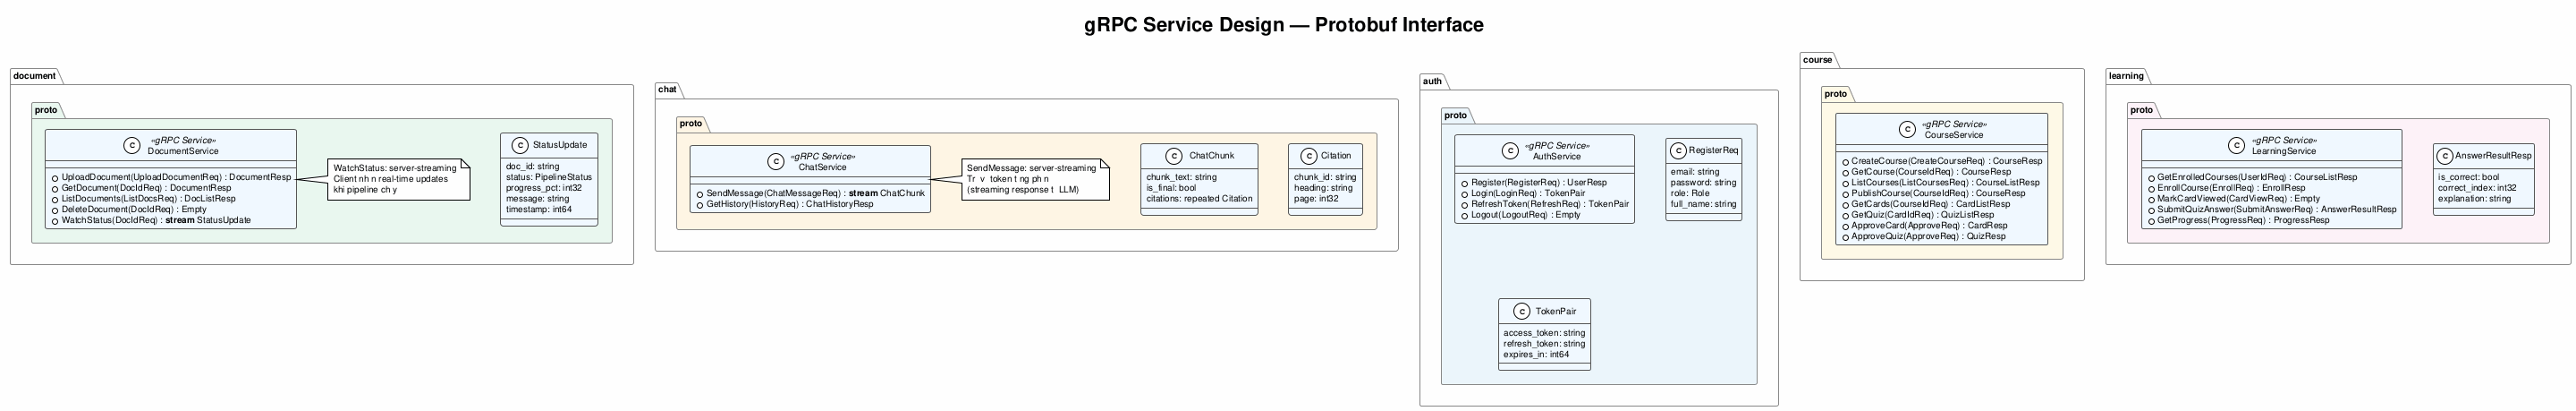
\includegraphics[width=0.95\textwidth]{diagrams/grpc_service_design.png}
    \caption{Thiết kế gRPC service và các use case tương ứng.}
    \label{fig:grpc-design-lvtn}
\end{figure}

\subsection{Internal Services}

Các nhóm service chính trong hệ thống gồm:
\begin{table}[H]
    \centering
    \caption{Các service chính trong kiến trúc triển khai.}
    \label{tab:services-lvtn}
    \begin{tabular}{p{3.5cm}p{10.5cm}}
        \toprule
        \textbf{Service} & \textbf{Vai trò} \\
        \midrule
        Next.js frontend & UI, LTI login/launch, proxy hoặc gọi API backend. \\
        Python gRPC service & API xử lý tài liệu, search, curriculum và quiz. \\
        Document worker & Parse, chunk, embed và lưu kết quả xử lý tài liệu. \\
        Enrichment worker & Sinh card/quiz bằng LLM và validate kết quả. \\
        Outbox worker & Đồng bộ sự kiện từ PostgreSQL sang Neo4j. \\
        PostgreSQL & Source of truth cho metadata, document, chunk, card, quiz và curriculum. \\
        Qdrant & Vector store phục vụ semantic search và retrieval. \\
        Neo4j & Knowledge Graph cho Course, Chapter, LO, Assessment và quan hệ SUPPORTS. \\
        MinIO & Object storage cho file gốc. \\
        Redis/Queue & Queue và trạng thái xử lý bất đồng bộ. \\
        \bottomrule
    \end{tabular}
\end{table}

\subsection{Async Workers}

Worker giúp tách tác vụ nặng khỏi request/response trực tiếp. Document worker
xử lý parse, chunk và embed; enrichment worker sinh nội dung học tập; outbox
worker đồng bộ dữ liệu sang graph. Các worker đọc job từ queue, cập nhật trạng
thái document và ghi log lỗi để người dùng có thể retry khi cần.

\subsection{Event / Queue Flow}

Sau khi upload thành công, backend tạo document ở trạng thái \texttt{QUEUED}
và enqueue job. Worker chuyển trạng thái qua các bước \texttt{PARSING},
\texttt{CHUNKING}, \texttt{EMBEDDING}, \texttt{GENERATING}, sau đó kết thúc
bằng \texttt{DONE} hoặc \texttt{ERROR}. Các sự kiện liên quan đến curriculum
và chunk-LO mapping được ghi vào outbox để đồng bộ sang Neo4j.

\section{Sequence Diagrams và System Flows}

\subsection{Luồng ingest curriculum}

\begin{figure}[H]
    \centering
    
\includegraphics[width=0.95\textwidth]{figures/seq_ingest_curriculum.png}
    \caption{Sequence diagram cho luồng ingest đề cương môn học.}
    \label{fig:seq-ingest-curriculum-lvtn}
\end{figure}

Luồng ingest curriculum bắt đầu từ request của giảng viên hoặc admin, sau đó
backend gọi parser để trích xuất Course, Chapter, Learning Outcome và
Assessment. Dữ liệu được lưu vào PostgreSQL trước, sau đó outbox/event
projector đồng bộ sang Neo4j. Thiết kế này giữ PostgreSQL làm source of truth
và cho phép Neo4j được rebuild nếu cần.

\subsection{Luồng xử lý tài liệu}

Luồng xử lý tài liệu gồm các bước upload, enqueue, parse, chunk, embed,
generate và persist. Các bước có thể retry độc lập ở cấp job. Trạng thái
document được cập nhật để frontend có thể hiển thị tiến trình cho giảng viên.

\begin{table}[H]
    \centering
    \caption{Trạng thái pipeline xử lý tài liệu.}
    \label{tab:pipeline-states-lvtn}
    \begin{tabular}{p{3cm}p{10.5cm}}
        \toprule
        \textbf{Trạng thái} & \textbf{Ý nghĩa} \\
        \midrule
        \texttt{QUEUED} & Document đã lưu và đang chờ worker xử lý. \\
        \texttt{PARSING} & Worker đang trích xuất text/metadata từ file. \\
        \texttt{CHUNKING} & Nội dung đang được chia thành chunk học tập. \\
        \texttt{EMBEDDING} & Chunk đang được chuyển thành vector. \\
        \texttt{GENERATING} & LLM đang sinh card/quiz. \\
        \texttt{DONE} & Pipeline hoàn tất thành công. \\
        \texttt{ERROR} & Pipeline thất bại sau số lần retry cho phép. \\
        \bottomrule
    \end{tabular}
\end{table}

\subsection{Luồng học và làm quiz}

Khi học viên mở tool từ LMS, hệ thống xác thực LTI launch và tạo session. Học
viên chỉ nhìn thấy nội dung đã publish. Khi làm quiz, submission được lưu cùng
score, đáp án đã chọn, thời điểm làm bài và context bài học. Dữ liệu này là
nền tảng cho dashboard học tập và recommendation/adaptive learning trong giai
đoạn sau.
